\documentclass[12pt]{article}

\usepackage[letterpaper, margin=1in]{geometry}
\usepackage{tikz}
\usetikzlibrary{calc}
\usepackage{enumitem}
\usepackage{graphicx}

\setlength{\parskip}{1em}
\setlength{\parindent}{0pt}

\begin{document}

\begin{titlepage}
    \centering
    \vfill
    \vspace*{2.5in}
    \begin{tikzpicture}[remember picture, overlay]
        \draw [line width=1pt] 
            ($(current page.north west) + (0.5in,-0.5in)$) rectangle 
            ($(current page.south east) + (-0.5in,0.5in)$);
    \end{tikzpicture}
    {\Huge\bfseries Capstone 2025 - Initial Proposal \par}
    \vspace{0.2in}
    {\LARGE Tolly Zhang \par}    
    \vspace{0.2in}
    {\LARGE December 20, 2024 \par}
    \vfill
\end{titlepage}

\newpage
\section*{Project Overview}
This project aims to develop an aerial package delivery system designed to transport small to medium-sized payloads over short to medium-range distances. The system will consist of four primary components:

\begin{enumerate}[label=\arabic*.] % Correct usage of enumerate
    \item \textbf{Dynamic Aerial Mobility System (DAMS)}  
    
    The DAMS will feature a Vertical Take-Off and Landing (VTOL) flight system, capable of switching between VTOL and fixed-wing flight modes. The VTOL mode will be used for takeoff and landing, while the fixed-wing mode will facilitate efficient cruising. The DAMS will be responsible for controlling the aircraft during flight, utilizing actuators and sensors for stability and maneuverability.
    
    \item \textbf{Payload Retrieval and Deployment Module (PRDM)}  
    
    The PRDM will be responsible for the autonomous retrieval and deployment of payloads. Key features will include:
    \begin{itemize}
        \item An opening/closing door for payload access.
        \item A clamp mechanism to securely hold the payload.
        \item A winch mechanism for raising and lowering the payload.
        \item Sensors to monitor weight distribution, providing real-time data to the DAMS to ensure stability and balance.
    \end{itemize}

    \item \textbf{Automated Flight Navigation System (AFNS)}  
    
    The AFNS will be responsible for determining the optimal flight path from the source to the destination, and providing navigational instructions to the DAMS. It will be capable of managing multiple aircraft simultaneously, enabling efficient coordination of deliveries.
    
    \item \textbf{Adaptive Flight Control Interface (ACFI)}  
    
    The ACFI will serve as the human-machine interface, allowing the operator to interact with both the AFNS and the DAMS. It will feature:
    \begin{itemize}
        \item Multiple modes of operation, including manual, semi-autonomous, and autonomous.
        \item Input devices such as screens, keyboards, mice, and controllers.
        \item A speech control interface for hands-free operation.
    \end{itemize}
\end{enumerate}

Each component will work together to ensure the system’s efficiency, autonomy, and ease of use for aerial package delivery operations.

\newpage

Below is a diagram of the proposed system architecture:

\noindent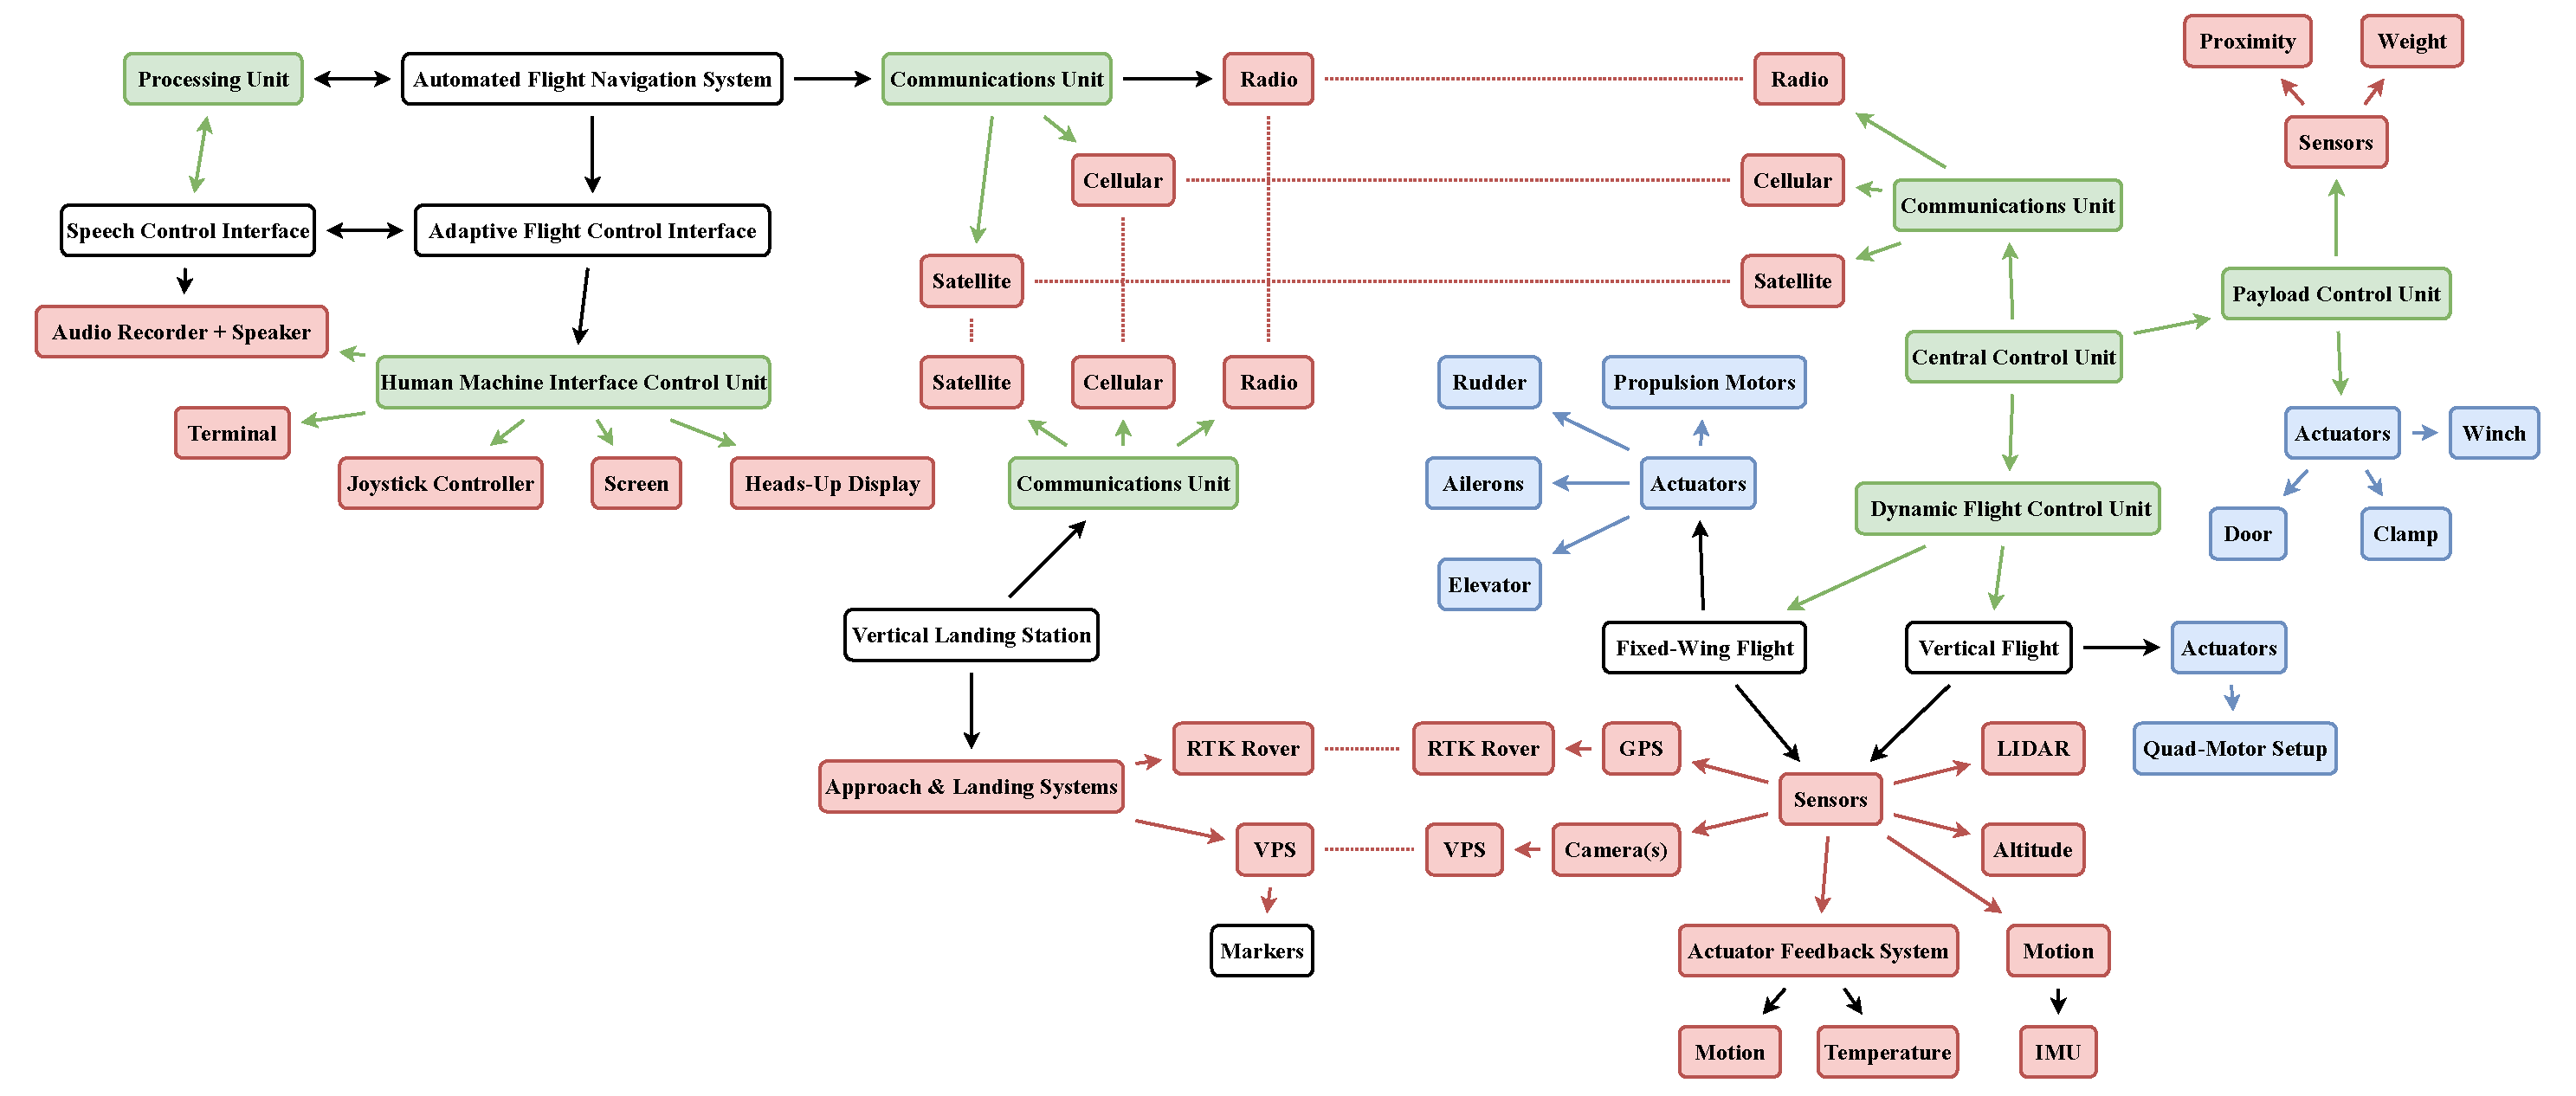
\includegraphics[width=\textwidth]{resources/system-architecture.drawio.pdf}

\end{document}
